\documentclass[stu, 12pt, letterpaper, donotrepeattitle, floatsintext, noapacite]{apa7}
\usepackage[utf8]{inputenc}
\usepackage[spanish, es-nodecimaldot, es-tabla]{babel}
\usepackage{csquotes}
\usepackage{hyperref}
\usepackage{graphicx}
\graphicspath{ {./attachtments/} }

% Configuración de bibliografía usando biblatex-apa
\usepackage[style=apa, sortcites=true, sorting=nyt, backend=biber]{biblatex}
\addbibresource{referencias.bib}

% Creación de archivo de referencias de ejemplo
\begin{filecontents}[overwrite]{referencias.bib}
@book{american2020publication,
  title={Publication manual of the American Psychological Association},
  author={{American Psychological Association}},
  year={2020},
  publisher={American Psychological Association},
  edition={7}
}

@article{ejemplo2023,
  title={Un artículo de ejemplo para el formato APA 7},
  author={Pérez, Juan and García, María},
  journal={Revista de Psicología General},
  volume={15},
  number={2},
  pages={123--135},
  year={2023},
  doi={10.1234/rpg.2023.001}
}
@online{ual2026,
  author={{Universidad de Almería}},
  title={Gestión de Memoria en Sistemas Operativos},
  url={https://w3.ual.es/~rguirado/so/tema5.pdf},
  urldate={2026-02-13}
}

@online{grokiseg,
  author={{Grokipedia}},
  title={Memory Segmentation Architecture},
  url={https://grokipedia.com/page/Memory_segmentation},
  urldate={2026-02-13}
}

@online{grokipage,
  author={{Grokipedia}},
  title={Memory Paging Mechanisms},
  url={https://grokipedia.com/page/Memory_paging},
  urldate={2026-02-13}
}

@online{analisis,
  author={{Análisis Multimedia}},
  title={Segmentación de Memoria y Ciclos de CPU},
  url={https://www.youtube.com/watch?v=p9yZNLeOj4s},
  urldate={2026-02-13}
}
\end{filecontents}

% Información del documento
\title{Actividad 3}
\author{Fernando Israel Rios Garcia-AL02877016@tecmilenio.mx \\
Artur Mikhail Lazurenko Mannanov-AL03028732@tecmilenio.mx \\
Angel Cuevas Lopez-AL03033114@tecmilenio.mx}
\affiliation{Universidad Tecmilenio}
\course{LSTI2308: Sistemas Operativos}
\professor{Ana Cruz}
\duedate{\today}

\begin{document}

% 1. Portada (Se genera automáticamente con \maketitle en apa7 modo stu)
\maketitle

% 2. Tabla de Contenidos
% APA 7 no requiere obligatoriamente una tabla de contenidos para trabajos estudiantiles,
% pero se incluye aquí como solicitado. Aseguramos que se muestren los niveles.
\setcounter{tocdepth}{3}
\setcounter{secnumdepth}{3}
\tableofcontents
\listoffigures
\newpage

% 3. Cuerpo del Documento
% 3. Cuerpo del Documento
\section{Introducción}
Este documento presenta el desarrollo de la Actividad 3, abordando temas clave en sistemas operativos como la administración de memoria, el diseño de sistemas de archivos, algoritmos de planificación de disco y almacenamiento RAID. Se incluyen propuestas técnicas, análisis prácticos y simulaciones para demostrar la comprensión de estos conceptos.

\section{Parte 1: Análisis de la administración de la memoria}

\subsection{Propuesta Técnica: Implementación de Segmentación}

\subsubsection{Introducción}
Esta propuesta define el mecanismo de gestión de memoria principal para un sistema operativo diseñado para entornos de alta eficiencia. Se selecciona la segmentación como esquema fundamental, permitiendo que el sistema gestione la memoria basándose en la visión lógica del programador y la estructura natural de los procesos.

\subsubsection{Modelo de Gestión de Memoria}
A diferencia de sistemas operativos robustos y complejos (monolíticos tradicionales), este núcleo se orienta a la eficiencia mediante tareas particulares y una estructura simplificada.

\textbf{Eficiencia de Segmentos:} El sistema es veloz en el uso de memoria debido a una segmentación correcta de los programas. El cargador del SO respeta la división lógica (código, datos, pila) establecida durante la compilación.

\textbf{Estrategia de Asignación:} Se requiere un análisis previo del espacio necesario para cada segmento. El núcleo utiliza esta información para minimizar el desperdicio y optimizar el tiempo de respuesta del gestor de memoria.

\begin{figure}[h]
    \centering
    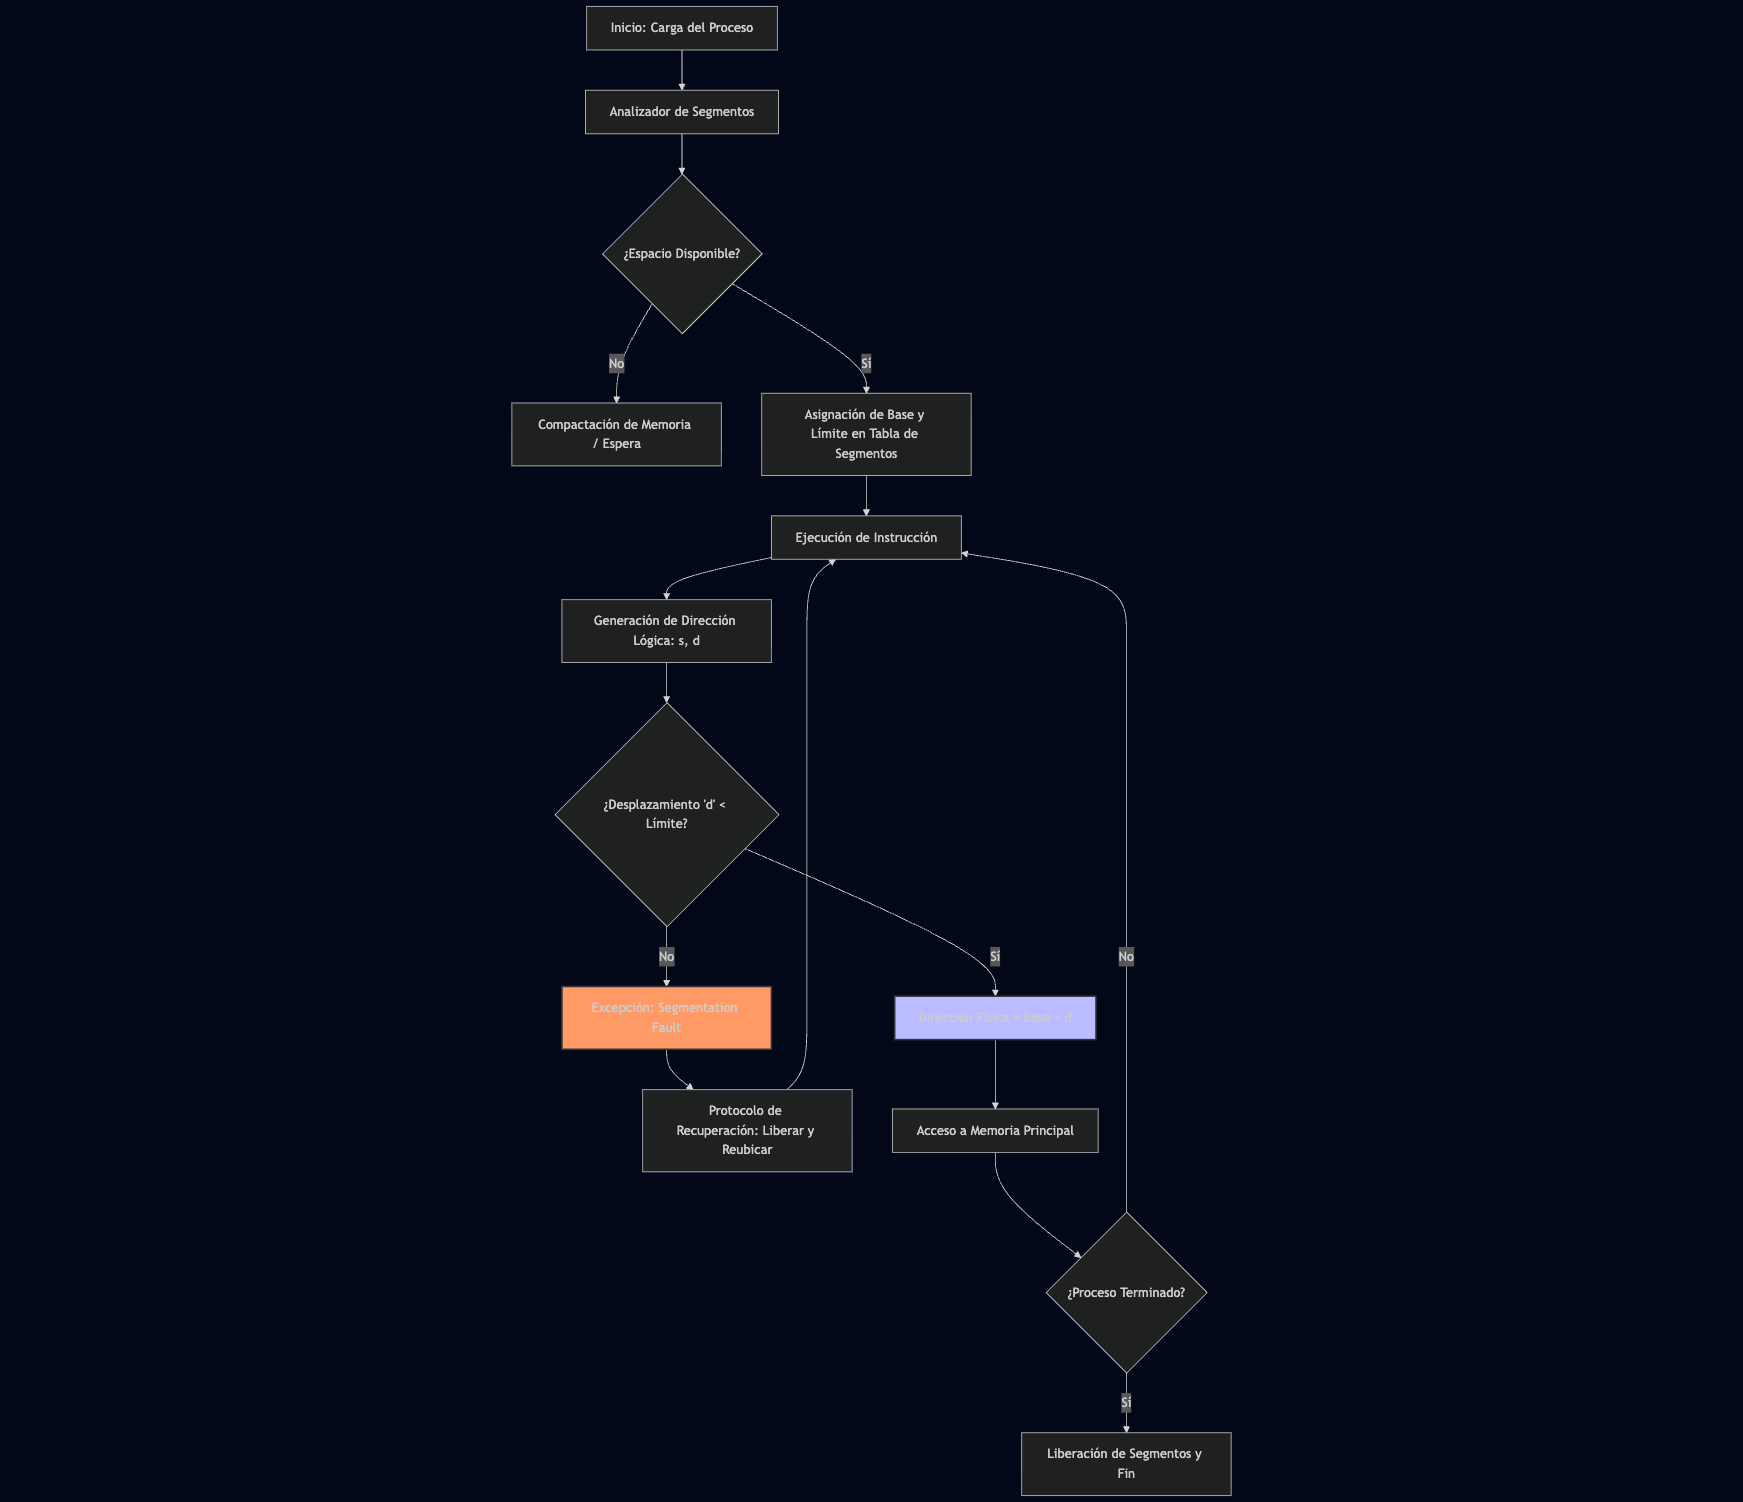
\includegraphics[width=0.8\textwidth]{part1.png}
    \caption{Diagrama de Segmentación de Memoria}
    \label{fig:part1}
\end{figure}

\subsubsection{Análisis de Etapas Operativas}

\paragraph{Etapa 1: Planificación de la Tabla de Segmentos}
El sistema operativo establece una Tabla de Segmentos para cada proceso. El análisis previo permite definir la base y el límite de cada entrada, asegurando que la protección de memoria sea estricta y el aprovechamiento del espacio sea máximo.

\paragraph{Etapa 2: Traducción y Ejecución}
Durante la ejecución de procesos, la unidad de gestión de memoria utiliza la segmentación para acceder a instrucciones de forma inmediata. Al ser un sistema diseñado para tareas particulares, se evitan las latencias de estructuras de paginación multinivel, favoreciendo la velocidad bruta.

\paragraph{Etapa 3: Control de Restricciones y Excepciones}
Dada la naturaleza de la segmentación en un entorno de memoria limitada:
\begin{itemize}
    \item \textbf{Fragmentación Externa:} El núcleo gestiona la fragmentación externa derivada de la asignación de bloques de tamaño variable.
    \item \textbf{Gestión de Violación de Límites:} Cuando un cálculo de dirección lógica excede el límite definido en la partición del segmento, el hardware genera una excepción de segmentación (Segmentation Fault).
\end{itemize}

\subsubsection{Protocolo de Recuperación del Sistema}
Ante el fallo de un proceso por exceso de límite de segmento, el núcleo ejecuta el siguiente protocolo de recuperación:
\begin{enumerate}
    \item Interrupción del proceso mediante excepción de protección.
    \item Liberación de los marcos de memoria comprometidos.
    \item Recarga de los segmentos en la memoria principal (reubicación si es necesario).
    \item Reinicio de la ejecución del proceso para restaurar el servicio.
\end{enumerate}

\subsubsection{Referencias Bibliográficas}
Para la elaboración de esta propuesta se consultaron las siguientes fuentes \cite{ual2026, grokiseg, grokipage, analisis}.

\section{Parte 2: Diseño y organización del sistema de archivos}

\subsection{Exploración práctica}
En esta actividad se exploraron comandos y directorios clave en un entorno Linux.

\subsubsection{Comandos utilizados}
\begin{itemize}
    \item \texttt{pwd}: Muestra la ruta del directorio actual.
    \item \texttt{ls}: Lista el contenido de directorios. \texttt{ls -l} para detalles y permisos, \texttt{ls -a} para archivos ocultos.
    \item \texttt{cd}: Cambiar de directorio (e.g., \texttt{cd /}, \texttt{cd /home}).
    \item \texttt{tree}: Ver estructura jerárquica (requiere instalación: \texttt{sudo apt install tree}).
\end{itemize}

\subsubsection{Directorios importantes del sistema Linux}
\begin{enumerate}
    \item \textbf{/ (root):} Raíz del sistema de archivos, inicio de toda la jerarquía.
    \item \textbf{/home:} Archivos personales de los usuarios.
    \item \textbf{/etc:} Archivos de configuración del sistema (red, usuarios, servicios).
    \item \textbf{/var:} Archivos variables como logs, caché, bases de datos temporales.
    \item \textbf{/bin:} Programas esenciales y comandos básicos (\texttt{ls}, \texttt{cp}, \texttt{rm}).
\end{enumerate}

\subsection{Actividad de diseño: Servidor CMS}
\textbf{Objetivo:} Crear un sistema que soporte múltiples sitios web, mantenga la separación de datos, sea seguro y fácil de administrar.

\subsubsection{Diagrama de estructura propuesta}
\begin{verbatim}
/
+-- cms
|   +-- sites
|   |   +-- sitio1 (public_html, config, logs, uploads, backups)
|   |   +-- sitio2 (public_html, config, logs, uploads, backups)
|   +-- shared (templates, plugins, libraries)
|   +-- database
|   +-- admin (scripts)
\end{verbatim}

\subsubsection{Organización de archivos y directorios}
\begin{itemize}
    \item \textbf{/cms/sites/:} Contiene espacios independientes para cada sitio web.
    \begin{itemize}
        \item \texttt{public\_html}: Archivos visibles (HTML, CSS, JS).
        \item \texttt{config}: Configuración privada (conexión BD), no accesible públicamente.
        \item \texttt{logs, uploads, backups}: Registros, subidas y copias de seguridad aisladas.
    \end{itemize}
    \item \textbf{/cms/shared/:} Recursos compartidos para evitar duplicidad (plantillas, plugins).
    \item \textbf{/cms/database/:} Archivos de base de datos con acceso restringido.
    \item \textbf{/cms/admin/:} Scripts de mantenimiento y administración.
\end{itemize}

\subsubsection{Configuración de permisos y seguridad}
Se utiliza el sistema de permisos Linux (r, w, x) y usuarios específicos:
\begin{itemize}
    \item \textbf{Usuarios/Grupos:} \texttt{admin} (administrador), \texttt{web\_sitio1}, \texttt{web\_sitio2}, grupo \texttt{cms\_sites}.
    \item \textbf{Permisos recomendados:}
    \begin{itemize}
        \item Sitios: \texttt{chmod 750} (Dueño control total, Grupo acceso limitado).
        \item \texttt{public\_html}: \texttt{chmod 755} (Lectura pública).
        \item \texttt{config}, \texttt{database}: \texttt{chmod 700} (Solo propietario).
        \item \texttt{shared}: \texttt{chmod 755} (Solo lectura para sitios).
    \end{itemize}
\end{itemize}

\textbf{Medidas de seguridad:} Separación de datos por usuarios, restricción de permisos en archivos sensibles, copias de seguridad automáticas y registro de actividad en logs.

\section{Parte 3: Simulación de algoritmos de planificación del disco}

\subsection{Resultados de la simulación}
Se implementó una simulación para los algoritmos FCFS, SSTF y SCAN con la secuencia de solicitudes: 95, 180, 34, 119, 11, 123, 62, 64 (Inicio: 50).

\subsubsection{FCFS (First-Come, First-Served)}
\textbf{Orden de atención:} 50 $\rightarrow$ 95 $\rightarrow$ 180 $\rightarrow$ 34 $\rightarrow$ 119 $\rightarrow$ 11 $\rightarrow$ 123 $\rightarrow$ 62 $\rightarrow$ 64 \\
\textbf{Movimiento total:} 644 pistas.

\begin{figure}[h]
    \centering
    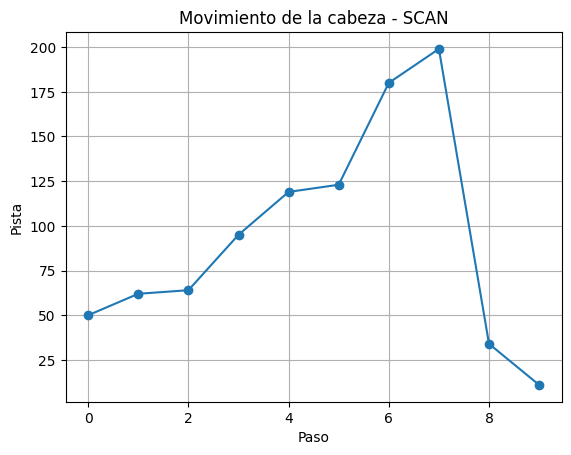
\includegraphics[width=0.7\textwidth]{part3.fig1.png}
    \caption{Gráfico de movimiento FCFS}
\end{figure}

\subsubsection{SSTF (Shortest Seek Time First)}
\textbf{Orden de atención:} 50 $\rightarrow$ 62 $\rightarrow$ 64 $\rightarrow$ 34 $\rightarrow$ 11 $\rightarrow$ 95 $\rightarrow$ 119 $\rightarrow$ 123 $\rightarrow$ 180 \\
\textbf{Movimiento total:} 236 pistas.

\begin{figure}[h]
    \centering
    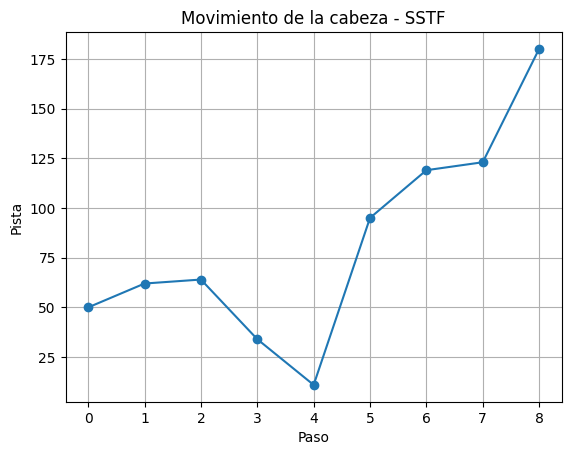
\includegraphics[width=0.7\textwidth]{part3.fig2.png}
    \caption{Gráfico de movimiento SSTF}
\end{figure}

\subsubsection{SCAN (Elevator Algorithm)}
\textbf{Orden de atención (hacia la derecha):} 50 $\rightarrow$ 62 $\rightarrow$ 64 $\rightarrow$ 95 $\rightarrow$ 119 $\rightarrow$ 123 $\rightarrow$ 180 $\rightarrow$ 199 $\rightarrow$ 34 $\rightarrow$ 11 \\
\textbf{Movimiento total:} 337 pistas.

\begin{figure}[h]
    \centering
    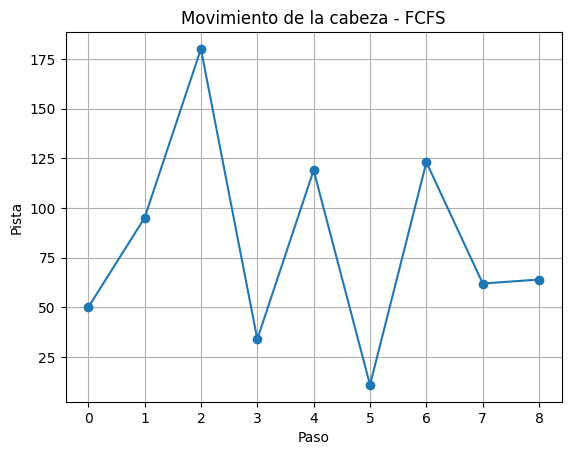
\includegraphics[width=0.7\textwidth]{part3.fig3.png}
    \caption{Gráfico de movimiento SCAN}
\end{figure}

\subsection{Análisis}
El algoritmo \textbf{SSTF} resultó ser el más eficiente en este caso con un movimiento total de 236 pistas, minimizando el tiempo de búsqueda al atender siempre la solicitud más cercana. FCFS, aunque garantiza justicia, resultó en el mayor movimiento (644). SCAN ofrece un compromiso intermedio (337) y es más predecible que SSTF en cargas altas.

\section{Parte 4: Configuración y análisis de RAID en Linux}

\subsection{Práctica en Linux: Configuración de RAID}
Se utilizaron discos virtuales (\texttt{/dev/sdb}, \texttt{/dev/sdc}) y la herramienta \texttt{mdadm}.

\subsubsection{RAID 0 (Striping)}
\begin{itemize}
    \item \textbf{Creación:} \texttt{sudo mdadm --create --verbose /dev/md0 --level=0 --raid-devices=2 /dev/sdb /dev/sdc}
    \item \textbf{Características:} Divide datos entre discos, ofreciendo mayor velocidad pero sin tolerancia a fallos.
    \item \textbf{Rendimiento (simulado):} Escritura $\approx$ 450 MB/s, Lectura $\approx$ 520 MB/s.
\end{itemize}

\subsubsection{RAID 1 (Mirroring)}
\begin{itemize}
    \item \textbf{Creación:} \texttt{sudo mdadm --create --verbose /dev/md1 --level=1 --raid-devices=2 /dev/sdb /dev/sdc}
    \item \textbf{Características:} Crea una copia exacta (espejo). Alta tolerancia a fallos, menor velocidad de escritura.
    \item \textbf{Prueba de fallo:} Se simuló fallo en \texttt{/dev/sdb} (\texttt{--fail}, \texttt{--remove}) y el sistema continuó funcionando correctamente.
    \item \textbf{Rendimiento (simulado):} Escritura $\approx$ 210 MB/s, Lectura $\approx$ 240 MB/s.
\end{itemize}

\subsection{Análisis comparativo}
\begin{itemize}
    \item \textbf{RAID 0:} Ideal para edición multimedia y datos temporales donde la velocidad es crítica. Riesgo alto de pérdida de datos.
    \item \textbf{RAID 1:} Recomendado para servidores web y bases de datos donde la integridad y disponibilidad son prioritarias.
\end{itemize}

\section{Parte 5: Informe final}
En esta actividad integradora se abarcaron aspectos esenciales de la administración de sistemas. Se diseñó una estrategia de segmentación para memoria embebida, priorizando la eficiencia. Se estructuró un sistema de archivos seguro para un CMS, aplicando permisos granulares. Se demostró mediante simulación que algoritmos como SSTF optimizan el movimiento del disco frente a FCFS. Finalmente, la implementación de RAID corroboró las compensaciones teóricas entre rendimiento (RAID 0) y redundancia (RAID 1), permitiendo seleccionar la configuración adecuada según la criticidad de los datos.

\newpage

% 4. Referencias
\printbibliography[title={Referencias}]

\end{document}
